\subsection{Modeling the solar energy curve} \label{sec:solar_energy_curve}
To further estimate the electrical energy yield of a PV generator which is inclined with the angle $\beta$, the Sun's radiation flux $\Phi_{\mathrm{G}}$ onto its energy-converting area $A_{\mathrm{PV}}$ must be modeled over the course of one day. Since the Sun's irradiance is symmetrical for $t_0 = 12\mathrm{h}$ and the PV generator is assumed to be aligned so that $A_{\mathrm{PV}}$ is perpendicular to the Sun's rays for $t_0 = 12\mathrm{h}$, the Sun's radiation flux $\Phi_{\mathrm{G}}$ as a Gaussian function of the solar time $t_{\mathrm{S}}$ can be approximated as shown in the figure \ref{fig:tikz_energy_gauss}.
\begin{figure}[h!]
	\centering
	

\tikzset{every picture/.style={line width=0.75pt}} %set default line width to 0.75pt        

\begin{tikzpicture}[x=0.75pt,y=0.75pt,yscale=-1,xscale=1]
%uncomment if require: \path (0,300); %set diagram left start at 0, and has height of 300

%Image [id:dp32150908690987645] 
\draw (327,150) node  {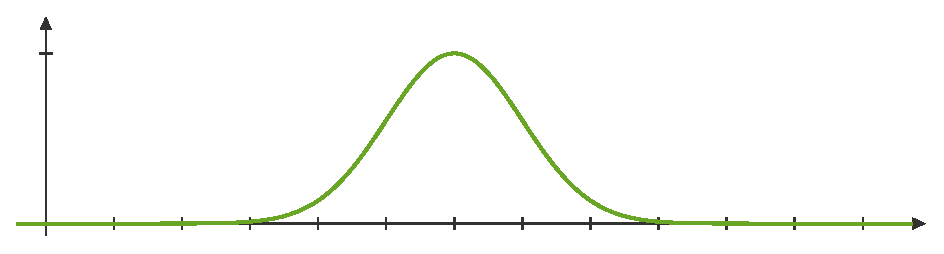
\includegraphics[width=439.5pt,height=105pt]{images/image_energy_gauss}};
%Straight Lines [id:da07666169968429992] 
\draw [color={rgb, 255:red, 155; green, 155; blue, 155 }  ,draw opacity=1 ] [dash pattern={on 4.5pt off 4.5pt}]  (63,103.4) -- (306,103.4) ;
%Straight Lines [id:da12384412498194441] 
\draw [color={rgb, 255:red, 155; green, 155; blue, 155 }  ,draw opacity=1 ] [dash pattern={on 4.5pt off 4.5pt}]  (315.6,201) -- (315.6,103) ;
%Shape: Circle [id:dp581375357919033] 
\draw  [fill={rgb, 255:red, 255; green, 255; blue, 255 }  ,fill opacity=1 ] (313.6,103.5) .. controls (313.6,102.4) and (314.5,101.5) .. (315.6,101.5) .. controls (316.7,101.5) and (317.6,102.4) .. (317.6,103.5) .. controls (317.6,104.6) and (316.7,105.5) .. (315.6,105.5) .. controls (314.5,105.5) and (313.6,104.6) .. (313.6,103.5) -- cycle ;

% Text Node
\draw (626,205.4) node [anchor=north west][inner sep=0.75pt]  [font=\footnotesize]  {$t_{\mathrm{S}}$};
% Text Node
\draw (34,59.4) node [anchor=north west][inner sep=0.75pt]  [font=\footnotesize]  {$\Phi _{\mathrm{G}}( t_{\mathrm{S}})$};
% Text Node
\draw (15,97.4) node [anchor=north west][inner sep=0.75pt]  [font=\footnotesize]  {$\Phi _{\mathrm{max}}$};
% Text Node
\draw (143,220.4) node [anchor=north west][inner sep=0.75pt]  [font=\footnotesize]  {$t_{\mathrm{S,r}} =t_{0} -3\tau _{\mathrm{S}}$};
% Text Node
\draw (162,240) node [anchor=north west][inner sep=0.75pt]  [font=\footnotesize] [align=left] {Sunrise};
% Text Node
\draw (298,240) node [anchor=north west][inner sep=0.75pt]  [font=\footnotesize] [align=left] {Noon};
% Text Node
\draw (287.5,220.4) node [anchor=north west][inner sep=0.75pt]  [font=\footnotesize]  {$t_{0} =12\mathrm{h}$};
% Text Node
\draw (403.1,220.4) node [anchor=north west][inner sep=0.75pt]  [font=\footnotesize]  {$t_{\mathrm{S,s}} =t_{0} +3\tau _{\mathrm{S}}$};
% Text Node
\draw (424,240) node [anchor=north west][inner sep=0.75pt]  [font=\footnotesize] [align=left] {Sunset};
% Text Node
\draw (564,220.4) node [anchor=north west][inner sep=0.75pt]  [font=\footnotesize]  {$2t_{0}$};
% Text Node
\draw (551,240) node [anchor=north west][inner sep=0.75pt]  [font=\footnotesize] [align=left] {Midnight};
% Text Node
\draw (44,220.4) node [anchor=north west][inner sep=0.75pt]  [font=\footnotesize]  {$0\mathrm{h}$};
% Text Node
\draw (14,240) node [anchor=north west][inner sep=0.75pt]  [font=\footnotesize] [align=left] {New solar day};


\end{tikzpicture}



	\caption{Model of the Sun's radiation flux $\Phi_{\mathrm{G}}$ onto the energy-converting area of a photovoltaic generator as a Gaussain function of the solar time $t_{\mathrm{S}}$. It is assumed that the Sun's irradiance is symmetrical around solar noon, and that the photovoltaic generator is aligned so that its energy-converting area is perpendicular to the Sun's rays at solar noon.}
	\label{fig:tikz_energy_gauss}
\end{figure}
The corresponding Gaussian function can be obtained from equation (\ref{eq:phi_gen_gauss}):
	\begin{equation} \label{eq:phi_gen_gauss}
	\centering
		\begin{gathered}
		\Phi_{\mathrm{G}}\left(t_{\mathrm{S}}\right) = \Phi_{\mathrm{max}} \, \exp\left(-\frac{(t_{\mathrm{S}} - t_0)^2}{2 \tau_\mathrm{S}^2}\right) \text{, } 
		\\
		\tau_\mathrm{S} = \frac{t_0 - t_{\mathrm{S,r}}}{3} = \frac{t_{\mathrm{S,s}} - t_0}{3} \text{.}
		\end{gathered}
	\end{equation}
The area this curve encloses with the solar time axis $t_{\mathrm{S}}$, from solar sunrise $t_{\mathrm{S,r}}$ to solar sunset $t_{\mathrm{S,s}}$, is equal to 99,7\% of the \emph{daily solar energy} $W_{\mathrm{G}}$ in $\left(\mathrm{Wh}\right)$ which occurs on the energy-converting area $A_{\mathrm{PV}}$ \cite{Landis:1995, Prechtl:2006, Prechtl:2008, Glover:2010, Schrufer:2014, AlNahhal:2019}:\footnote{$t_{\mathrm{S,r}}$ and $t_{\mathrm{S,s}}$ were selected this way for simplicity.}
	\begin{equation} \label{eq:w_gen_gauss}
	\centering
		W_\mathrm{G} = \frac{1}{0,997} \int\limits_{t_{\mathrm{S,r}}}^{t_{\mathrm{S,s}}} \Phi_{\mathrm{max}} \, \exp\left(-\frac{(t_{\mathrm{S}} - t_0)^2}{2 \tau_\mathrm{S}^2}\right) \,\mathrm{d}t_\mathrm{S} = \frac{\Phi_{\mathrm{max}} \, \tau_\mathrm{S} \sqrt{2\pi}}{0,997} \text{.}
	\end{equation}

A similar approach is used in \cite{Guo:2017, Nguyen:2020} and in \cite{Balafas:2010, Mertens:2015, Koudouris:2017} it can be seen that the Sun's total irradiance $E_{\mathrm{G}}$ throughout the day, from which $\Phi_{\mathrm{G}}$ derives, behaves similar to a Gaussian curve.\footnote{How to solve the integral in equation \ref{eq:w_gen_gauss} from $-\infty$ to $\infty$ can be found in the appendix \ref{sec:gauss_general}.}

The greates daily radiation flux $\Phi_{\mathrm{max}}$ in $\left(\mathrm W\right)$ onto $A_{\mathrm{PV}}$ can be calculated using the equations (\ref{eq:e_gen_ghi_dni}) and (\ref{eq:radiation_flux}) by deriving the following relationship:
	\begin{equation} \label{eq:w_gen}
	\centering
		W_\mathrm{G} = \int\limits_{t_{\mathrm{S,r}}}^{t_{\mathrm{S,s}}} \Phi_{\mathrm{G}}\,\mathrm{d}t_\mathrm{S} = A_{\mathrm{PV}} \int\limits_{t_{\mathrm{S,r}}}^{t_{\mathrm{S,s}}} E_{\mathrm{G}}\,\mathrm{d}t_\mathrm{S} \text{.}
	\end{equation}
Considering that $A_{\mathrm{PV}}$ is a constant factor and taking into account the findings from the subsection \ref{sec:energy_yield}, the integrals from equation (\ref{eq:w_gen}) can be partly solved as follows:
	\begin{equation} \label{eq:int_e_gen}
	\centering
		\begin{split}
		\int\limits_{t_{\mathrm{S,r}}}^{t_{\mathrm{S,s}}} E_{\mathrm{G}}\,\mathrm{d}t_\mathrm{S} = E_{\mathrm{GHI}} \left( \frac{1 + \cos \beta}{2} + \frac{1 - \cos \beta}{2} \cdot \mathrm{ALB} \right) \cdot \left(t_{\mathrm{S,s}} - t_{\mathrm{S,r}}\right) \\ 
		- E_{\mathrm{DNI}} \ \frac{1 + \cos \beta}{2} \underbrace{\int\limits_{t_{\mathrm{S,r}}}^{t_{\mathrm{S,s}}} \sin \gamma_{\mathrm{S}}\,\mathrm{d}t_\mathrm{S}}_\text{\textbf{\RN{1}}} + E_{\mathrm{DNI}} \underbrace{\int\limits_{t_{\mathrm{S,r}}}^{t_{\mathrm{S,s}}} \cos \theta \,\mathrm{d}t_\mathrm{S}}_\text{\textbf{\RN{2}}} \text{.}
		\end{split}
	\end{equation}
Using the equations (\ref{eq:sin_gamma_s}) and (\ref{eq:solar_hour_angle}), integral \text{\textbf{\RN{1}}} can be solved to:
	\begin{equation} \label{eq:int_rn_1}
	\centering
		\begin{aligned}
		\text{\textbf{\RN{1}}:} \ &\int\limits_{t_{\mathrm{S,r}}}^{t_{\mathrm{S,s}}} \sin \gamma_{\mathrm{S}}\,\mathrm{d}t_\mathrm{S} = 
		\sin \varphi \, \sin \delta \left(t_{\mathrm{S,s}} - t_{\mathrm{S,r}} \right) \\
		&+ c_{\varphi,\delta} \left(\sin \left(\left(t_{\mathrm{S,s}} - 12\mathrm{h} \right) \cdot \frac{15^\circ}{1\mathrm{h}} \right) - \sin \left(\left( t_{\mathrm{S,r}} - 12\mathrm{h} \right) \cdot \frac{15^\circ}{1\mathrm{h}} \right)\right) \text{,}
		\end{aligned}
	\end{equation}
with $c_{\varphi,\delta}$ being:
	\begin{equation} \label{eq:const_varphi_delta}
	\centering
		c_{\varphi,\delta} = \cos \varphi \, \cos \delta \cdot \frac{1\mathrm{h}}{15^\circ} \text{.}
	\end{equation}
Integral \text{\textbf{\RN{2}}} on the other hand cannot be solved analytically as easy. This is why a sum instead of an integral is used in the \MATLAB simulation (see appendix \ref{sec:matlab_code}) to calculate $W_{\mathrm{G}}$:
	\begin{equation} \label{eq:sum_energy}
	\centering
		W_\mathrm{G} = A_{\mathrm{PV}} \displaystyle\sum_{t_{\mathrm{S}} = t_{\mathrm{S,r}}}^{t_{\mathrm{S,s}}} E_{\mathrm{G}} \, \Delta t_{\mathrm{S}} \text{.}
	\end{equation}
Using trigonometric functions, $E_{\mathrm{G}}$ can be simplyfied as shown in the equation (\ref{eq:sum_e_gen}). Depending on the desired accuracy $\Delta t_{\mathrm{S}}$ in $\left( \mathrm{h} \right)$ can be smaller or greater. The smaller it is the more accurate $W_{\mathrm{G}}$ can be modeled.\footnote{$\Delta t_{\mathrm{S}}$ is one discrete time step of the solar time. It can be caluculated from the length $len$ of the Matlab vector that goes from $t_{\mathrm{S,r}}$ to $t_{\mathrm{S,s}}$: $\Delta t_{\mathrm{S}} = \frac{1}{len}$.}
	\begin{equation} \label{eq:sum_e_gen}
	\centering
		\begin{aligned}
		\displaystyle\sum_{t_{\mathrm{S}} = t_{\mathrm{S,r}}}^{t_{\mathrm{S,s}}} E_{\mathrm{G}} \, \Delta t_{\mathrm{S}} &= \displaystyle\sum_{t_{\mathrm{S}} = t_{\mathrm{S,r}}}^{t_{\mathrm{S,s}}} \left(E_{\mathrm{GHI}} - E_{\mathrm{DNI}} \, \sin \gamma_{\mathrm{S}} \right) \cos^2 \frac{\beta}{2} \, \Delta t_{\mathrm{S}} \\
		&+ \displaystyle\sum_{t_{\mathrm{S}} = t_{\mathrm{S,r}}}^{t_{\mathrm{S,s}}} \left(E_{\mathrm{DNI}} \, \cos \theta + E_{\mathrm{GHI}} \, \sin^2 \frac{\beta}{2} \cdot \mathrm{ALB} \right)\Delta t_{\mathrm{S}}
		\end{aligned}
	\end{equation}
By inserting the caluclated $W_{\mathrm{G}}$ from equation (\ref{eq:sum_energy}) into equation (\ref{eq:w_gen_gauss}) and transforming it, the greates daily radiation flux $\Phi_{\mathrm{max}}$ onto $A_{\mathrm{PV}}$, which in this model occurs for $t_0 = 12\mathrm{h}$, can be obtained \cite{Appelbaum:1992, Landis:1995, Prechtl:2006, Prechtl:2008}:
	\begin{equation} \label{eq:phi_max_sum}
	\centering
		\Phi_{\mathrm{max}} = \frac{0,997 \cdot A_{\mathrm{PV}}}{\tau_\mathrm{S} \sqrt{2\pi}} \displaystyle\sum_{t_{\mathrm{S}} = t_{\mathrm{S,r}}}^{t_{\mathrm{S,s}}} E_{\mathrm{G}} \, \Delta t_{\mathrm{S}} \text{.}
	\end{equation}
